\chapter{関連研究}
\section{○に関する関連研究}
\label{sec:2.1}
Naguriら\cite{naguri}の研究が挙げられる.
hogehoge

\section{○○に関する関連研究}
\label{sec:2.2}
hogehogeなアプローチとして様々な手法が報告されている.

Chiuら\cite{chiu1}は○○した.

\begin{figure}[h]
 \centering
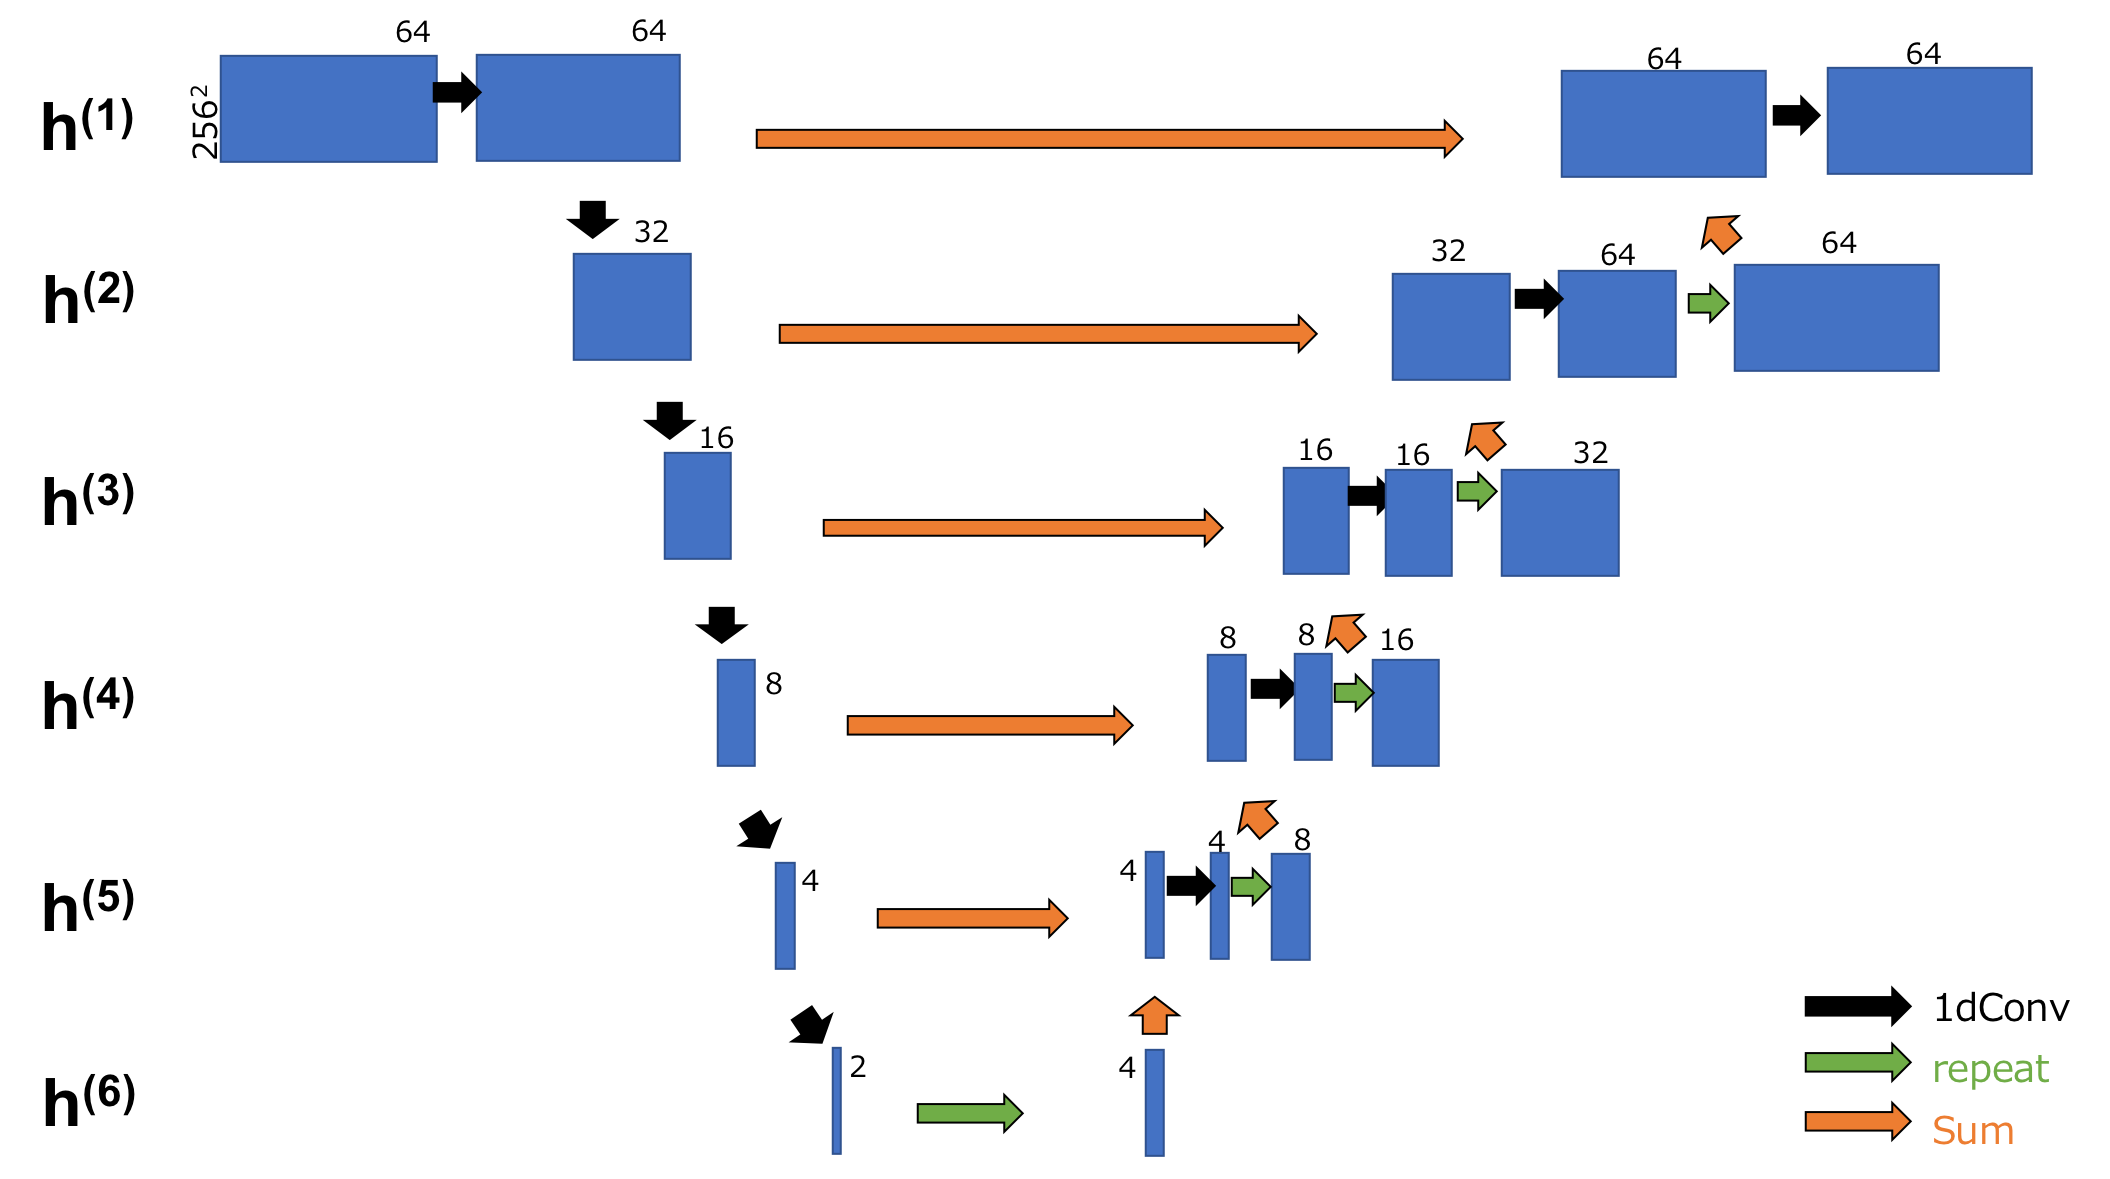
\includegraphics[keepaspectratio,width=103mm,height=77mm]{fig/net_example.png}
\caption{ネットワークの構造}
\label{fig:unet}
\end{figure}

\section{○○の応用研究}
\label{sec:2.3}
○○の応用研究として鈴木ら\cite{suzuki}の研究を紹介する.
